\section{Forsøg 2 - IKEA-oplader}

I dette forsøg undersøges sammenhængen mellem afstanden af oplader: senderen og telefonen: modtageren med henblik på tabet af energi når der sker en trådløs opladning, og afstanden mellem sender og modtager vokser. Altså effektiviteten $\eta$ undersøges ved forskellige afstande mellem sender og modtager.

\subsection{Forsøgsbeskrivelse}
\subsubsection{Komponenter}

\begin{table}[htbp] %% Komponenter tabel %%
\label{sender}
\begin{tabular}{l|l|c|l}
        & Powersupply                  & Oplader             & Cover               \\ \hline
Model:  & KMW-190-330-GS               & MORIK, E1404        & VITAHULT, 22974     \\
Input:  & 220-240V$\sim$50/60Hz, 0.18A & 19V$\sim$1.74A, 10W & 19V$\sim$1.74A, 10W \\
Output: & 19V$\sim$1.74A, 10W          & 5W                  & 5V, 1A             
\end{tabular}
\caption{Alt er aflæst direkte fra komponenternes labels.}
\end{table}

\begin{table}[htbp]
\label{table:batteri}
\begin{tabular}{l|lcl}
         & Iphone 4S &          &        \\ \hline
Batteri: & Li-Po     & 1432 mAh & 5.3 Wh
\end{tabular}
\caption{Aflæst fra \cite{batteri}}
\end{table}

Strømkilden er et standart ikke jordet, tobenet, europæisk væg stikkontakt, 230 volt.

Som modtager er der benyttet en \textbf{Iphone 4S}, \textit{Model A1431 \textcolor{red}{EMC 380B med FCC ID: BCG-E2380B, IC: 578C-E2380B.}} 
Denne enhed er udstyret med cover, model og egenskaber kan ses i tabel \ref{sender}. Her er det dog vigtigt at notere sig at telefonen er brugt, og er en ældre model (købt november 2011). Altså er batteriet ikke i fabriksny tilstand. Det er usikkert om dette har haft en relevant effekt på det udførte forsøg. Da dette kan have en effekt på hvordan batteriet lader. I forsøget er der antaget at opladningen sker lineært, mere om dette i følgende sektioner.

Ydermere er der benyttet papir til at lægge imellem mobilen med coveret og opladeren for at øge afstanden mellem dem, så det magnetiske felt forstyrres mindst muligt, og afstanden er holdt fast. 

\textcolor{red}{Indsæt billede af opstilling her} 

\subsubsection{Fremgangsmåde}

Udførelsen af forsøget er meget simpel, og består af to dele der gentages tre gange. Første del er at bestemme hvor højt modtager telefonen skal være løftet fra opladeren. Altså længden L bestemmes i cm, hvor positiv retning er væk fra opladeren. Anden del er at aflæse telefonens batteriprocent hvert tiende minut. Dette gentages med tre forskellige værdier for L, altså tre forskellige afstande.

Alle tre gange sikres der at koblingen ikke er ustabil. Hjælp til at opnå dette er en diode, i opladeren, der lyser konstant hvis koblingen er stabil. For at opnå denne stabile kobling placeres telefonen midt ovenpå opladeren, så spolerne i henholdsvis sender og modtager ligger direkte ovenpå hinanden. Hertil er der tegnet en rød streg på både oplader og cover, det det er muligt at afgøre at coveret ligger samme sted under hvert forsøg.

Første L værdi er valgt til 0 cm da dette teoretisk set burde være den optimale kobling mellem sender og modtager i et system designet til trådløs energioverførsel. Det ses også i den første graf der hvor $L = 0$ at denne opnår den højeste ladningsprocent. Det skal dog noteres at spolerne i sender og modtager ikke lægger præcist direkte ovenpå hinanden da der er et lag plastik og et gummikryds imellem. Disse antages ikke at have nogen effekt på opladningen. Længden L starter fra den hvide plastikskive med gummikrydset på opladeren, altså direkte ovenpå. Den præcise afstand mellem plastic og spole i senderen er ukendt. Det samme gælder i coverets ydre plastiklag, hvor dennes tykkelse og afstand mellem den og modtager spolen også er ukendt.

Tiden er målt hvert tiende minut (bilag \ref{bilag:forsg2}) og målt med en afvigelse på $\pm 10$ sekunder, hvilket burde være hurtigt nok til ikke at se en ændring i ladningsprocenten.

\subsubsection{Resultater}
Rå, ikke redigeret, data kan ses i bilag \ref{bilag:forsg2}. Disse data er benyttet til at opstille de følgende tre diagrammer:

%\begin{figure}[H] %% udkommenteret side om side grafer da de var for små
%	\centering
%	\begin{minipage}[b]{0.48\textwidth}
%	\centering
%	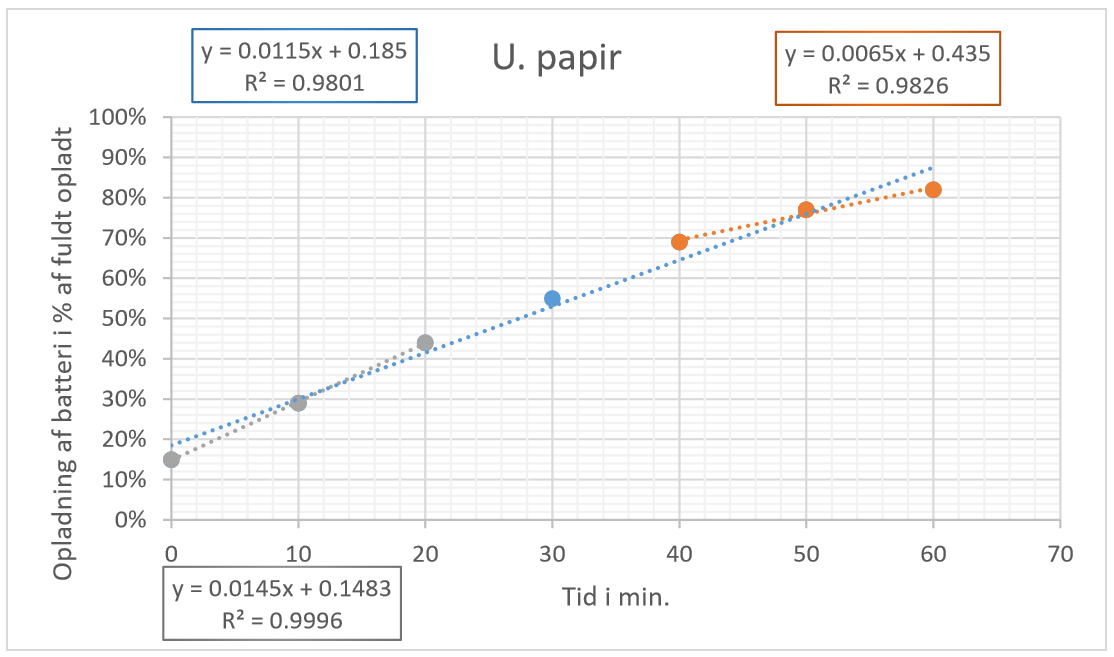
\includegraphics[width=1\textwidth]{Setup/forsg2_graf1} % Venstre billede
%	\end{minipage}
%	\hfill
%	\begin{minipage}[b]{0.5\textwidth}
%	\centering
%	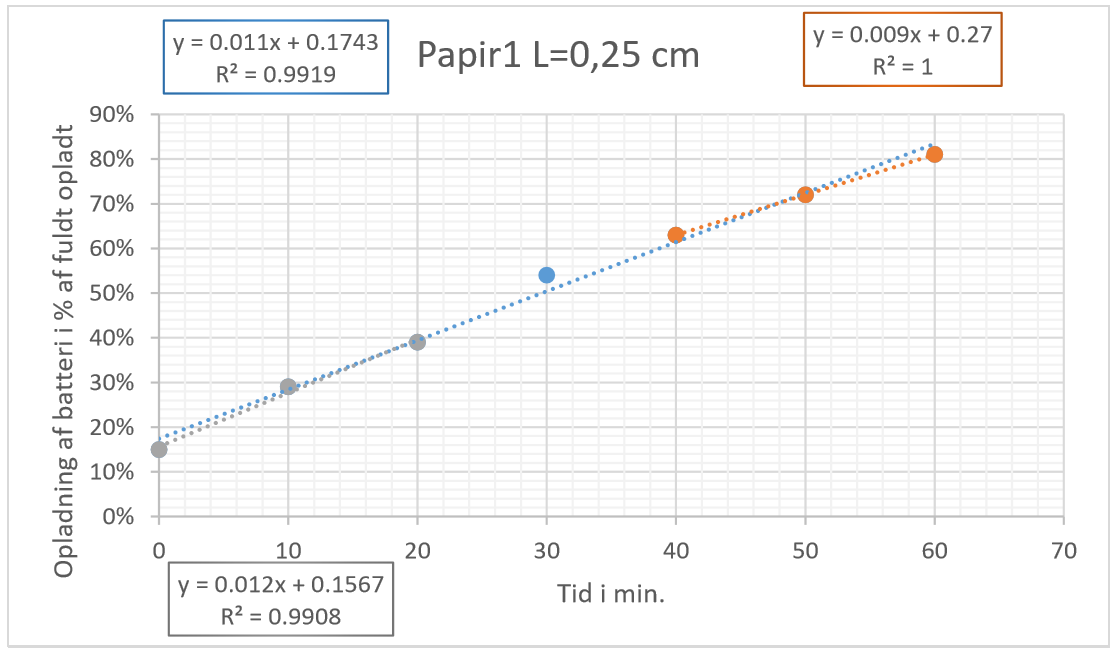
\includegraphics[width=1\textwidth]{Setup/forsg2_graf2} % Højre billede
%	\end{minipage}
%	\\ % Figurtekster og labels
%	\begin{minipage}[t]{0.5\textwidth}
%	\caption{} % Venstre figurtekst og label
%	\label{figure:graf1}
%	\end{minipage}
%	\hfill
%	\begin{minipage}[t]{0.48\textwidth}
%	\caption{} % Højre figurtekst og label
%	\label{figure:graf2}
%	\end{minipage}
%\end{figure}

\begin{figure}[H]
\centering
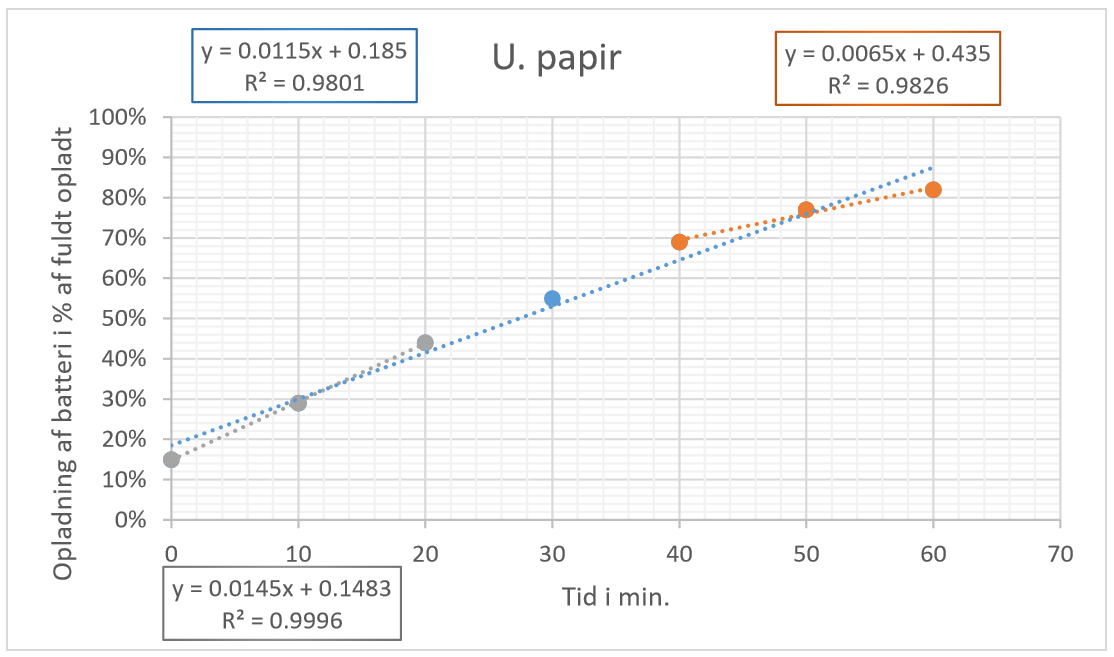
\includegraphics[width=1\textwidth]{Setup/forsg2_graf1}
\label{figure:graf1}
\caption{}
\end{figure}

\begin{figure}[H]
\centering
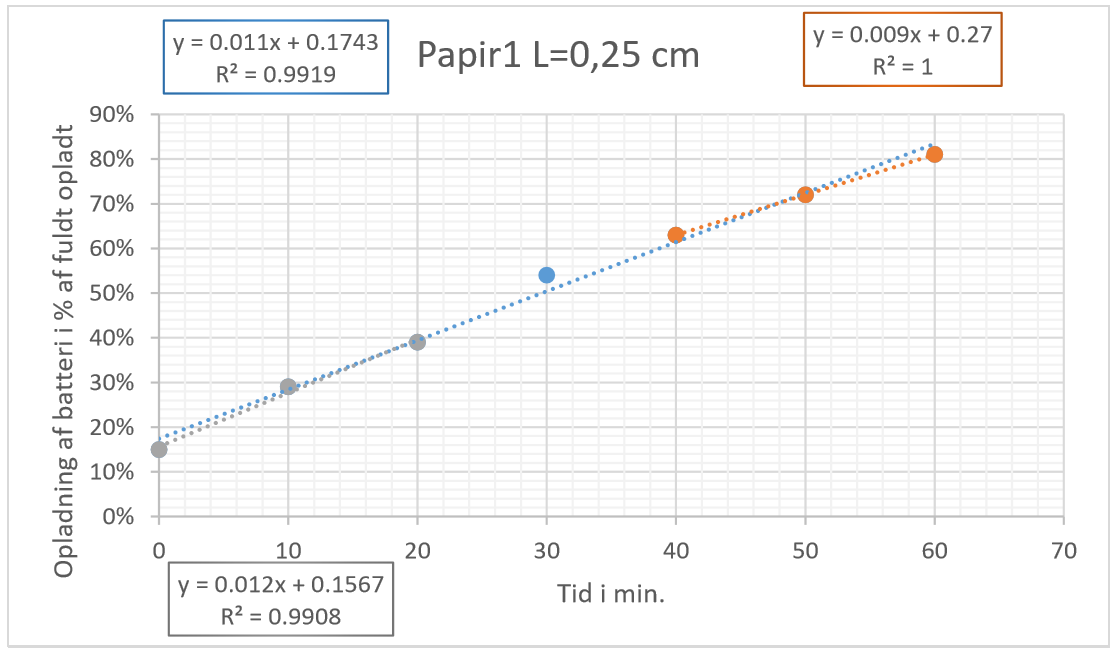
\includegraphics[width=1\textwidth]{Setup/forsg2_graf2}
\label{figure:graf2}
\caption{}
\end{figure}

\begin{figure}[H]
\centering
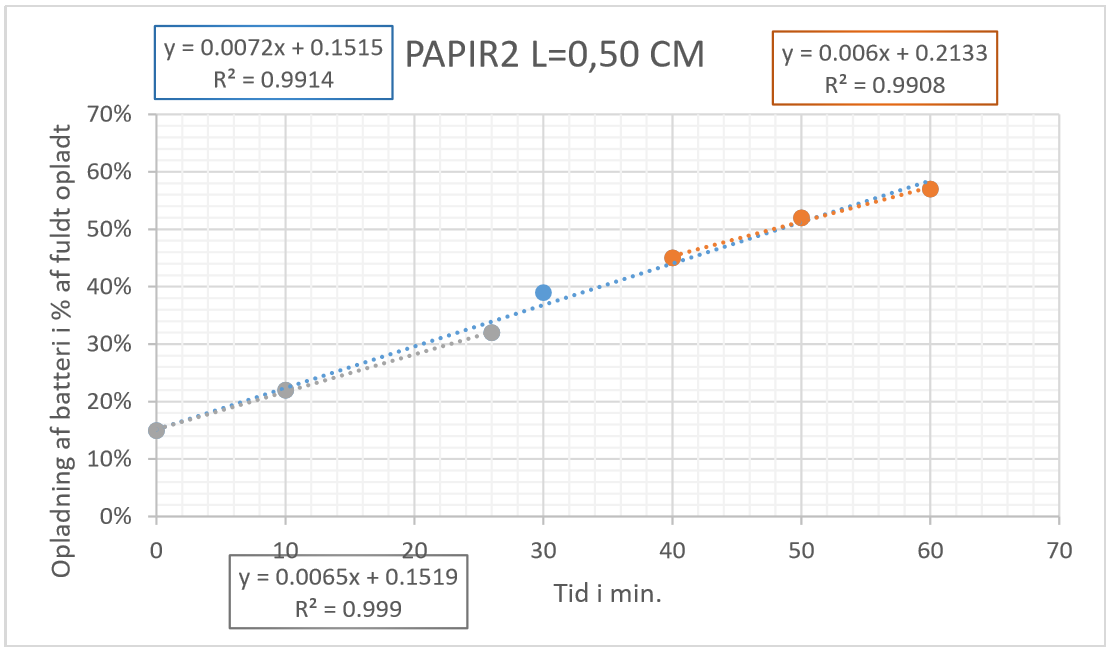
\includegraphics[width=1\textwidth]{Setup/forsg2_graf3}
\label{figure:graf3}
\caption{}
\end{figure}

\newpage

I første forsøg hvor $L = 0$ ses det at opladning af batteriet nåede op på 82 procent ladning af maksimal ladning på batteriet (100 procent), indenfor den målte tidsperiode på 60 minutter. I de to næste forsøg ender opladningsprocenten efter 60 minutter på henholdsvis 81 procent og 57 procent ved $L = 0.25$ og $L = 0.5$ aflæst fra figur \ref{figure:graf1} figur, \ref{figure:graf2} og figur \ref{figure:graf3}.

